\section{Bonus : hyperélasticité et potentiel neuronal}\label{sec:hyper}

\subsection{Rappels de grandes déformations}

On quitte l'hypothèse des petites perturbations. Le mouvement $\mathbf{x}=\bs\varphi(\mathbf{X})$ envoie la configuration de référence sur la configuration actuelle. On définit le gradient de la transformation $\F$, la variation de volume $J$, le tenseur de Cauchy--Green droit $\mathbf{C}$ et ses invariants :
\begin{align*}
&\F = \frac{\partial\mathbf{x}}{\partial\mathbf{X}}, && J=\det\F>0,\\
&\mathbf{C}=\F^T\F \ \text{(Cauchy--Green droit)}, && I_1=\tr\mathbf{C},\quad I_2=\tfrac12\big[(\tr\mathbf{C})^2-\tr(\mathbf{C}^2)\big],\quad I_3=\det\mathbf{C}=J^2.
\end{align*}
$\mathbf{C}$ ne dépend pas d'une rotation superposée ($\F\to\mathbf{Q}\F$ laisse $\mathbf{C}$ invariant). Il mesure donc la déformation « pure ». Pour un étirement diagonal $\F=\mathrm{diag}(\lambda_1,\lambda_2,\lambda_3)$, on a $I_1=\sum\lambda_i^2$ et $I_2=\sum_{i<j}\lambda_i^2\lambda_j^2$.

\paragraph{Hyperélasticité.} Un matériau est hyperélastique s'il existe une énergie libre $\psi(\F)$ par unité de volume de référence telle que la contrainte nominale (premier tenseur de Piola--Kirchhoff) soit
\begin{equation}
\Pk = \frac{\partial\psi}{\partial\F},\qquad \sig = J^{-1}\Pk\F^T,\qquad \mathbb{A}=\frac{\partial^2\psi}{\partial\F\,\partial\F}.
\end{equation}
\emph{Objectivité} : $\psi(\mathbf{Q}\F)=\psi(\F)$ pour toute rotation $\mathbf{Q}$, ce qui impose que $\psi$ ne dépende que de $\mathbf{C}$. \emph{Isotropie} : $\psi$ ne dépend alors que de $(I_1,I_2,J)$. $\mathbb{A}$ a toujours la symétrie majeure, puisque c'est une hessienne.

\subsection{Neo-Hooke compressible : la dérivation devient inutile}

\begin{equation}
\psi(\F) = \frac\mu2\big(I_1-3-2\ln J\big)+\frac\lambda2(\ln J)^2.
\end{equation}
Avec $\partial I_1/\partial\F=2\F$ et $\partial J/\partial\F=J\F^{-T}$, la dérivation à la main donne
\begin{align}
\Pk &= \mu(\F-\F^{-T})+\lambda\ln J\,\F^{-T},\\
\mathbb{A}_{iJkL} &= \mu\,\delta_{ik}\delta_{JL} + (\mu-\lambda\ln J)\,F^{-1}_{Li}F^{-1}_{Jk} + \lambda\,F^{-1}_{Ji}F^{-1}_{Lk}.
\end{align}
Avec JAX, on écrit seulement $\psi$ :
\begin{lstlisting}
def psi_neo_hooke(F, mu, lam):
    I1 = jnp.sum(F * F); lnJ = jnp.log(jnp.linalg.det(F))
    return 0.5 * mu * (I1 - 3.0 - 2.0 * lnJ) + 0.5 * lam * lnJ**2

P = jax.grad(psi_neo_hooke)(F, mu, lam)        # 3x3
A = jax.hessian(psi_neo_hooke)(F, mu, lam)     # 3x3x3x3
\end{lstlisting}
Sur des $\F$ aléatoires, l'écart avec les formules analytiques est de $2\times10^{-16}$ pour $\Pk$ et de $10^{-15}$ pour $\mathbb{A}$. Les tests vérifient aussi $\Pk(\I)=\mathbf{0}$, la symétrie majeure de $\mathbb{A}$ et l'objectivité $\Pk(\mathbf{Q}\F)=\mathbf{Q}\Pk(\F)$. Ici $\F$ n'a pas de symétrie, donc dériver par rapport à la matrice $3\times3$ est correct : le piège de la section~\ref{sec:jax} ne concerne que les arguments symétriques.

\subsection{Incompressibilité et essais homogènes}

Le caoutchouc est quasi incompressible ($K/\mu\sim10^3$). On impose $J=1$ par un multiplicateur de Lagrange $p$, la pression :
\[
\tilde\psi = \psi(I_1,I_2)-p(J-1)\quad\Longrightarrow\quad \Pk = 2\psi_1\F + 2\psi_2\big(I_1\F-\F\mathbf{C}\big) - p\,\F^{-T},\qquad \psi_i=\frac{\partial\psi}{\partial I_i}.
\]
La pression n'est pas donnée par la loi : elle est fixée par les conditions aux limites. Pour les trois essais de Treloar, on la détermine par la condition de bord libre.

\paragraph{Traction uniaxiale (UT).} $\F=\mathrm{diag}(\lambda,\lambda^{-1/2},\lambda^{-1/2})$. La condition $P_{22}=0$ donne $p=2\psi_1\lambda^{-1}+2\psi_2(I_1\lambda^{-1}-\lambda^{-2})$. En reportant dans $P_{11}$ et en utilisant $I_1=\lambda^2+2\lambda^{-1}$ :
\begin{equation}
P_{\mathrm{UT}} = 2\big(\lambda-\lambda^{-2}\big)\big(\psi_1+\lambda^{-1}\psi_2\big).
\end{equation}
\paragraph{Équibiaxiale (ET)} ($\F=\mathrm{diag}(\lambda,\lambda,\lambda^{-2})$) et \textbf{cisaillement pur (PS)} ($\F=\mathrm{diag}(\lambda,1,\lambda^{-1})$). Le même calcul donne
\begin{equation}
P_{\mathrm{ET}} = 2\big(\lambda-\lambda^{-5}\big)\big(\psi_1+\lambda^2\psi_2\big),\qquad P_{\mathrm{PS}} = 2\big(\lambda-\lambda^{-3}\big)\big(\psi_1+\psi_2\big).
\end{equation}
Dans le code, $\psi_1$ et $\psi_2$ sont obtenues par \code{jax.grad} du potentiel, \emph{quel qu'il soit} : analytique ou réseau de neurones.

\subsection{Potentiels étudiés}

\begin{center}
\begin{tabular}{lll}
\toprule
Modèle & $\psi(I_1,I_2)$ & paramètres\\
\midrule
Neo-Hooke & $C_{10}(I_1-3)$ & 1\\
Mooney--Rivlin & $C_{10}(I_1-3)+C_{01}(I_2-3)$ & 2\\
Yeoh~\cite{yeoh1993} & $C_{10}(I_1-3)+C_{20}(I_1-3)^2+C_{30}(I_1-3)^3$ & 3\\
ICNN & réseau convexe en entrée, ci-dessous & 230\\
\bottomrule
\end{tabular}
\end{center}

\begin{rappel}{polyconvexité}
Pour qu'un problème d'hyperélasticité ait une solution (théorème de Ball~\cite{ball1977}), on demande que $\psi$ soit \emph{polyconvexe} : convexe en $(\F,\operatorname{cof}\F,\det\F)$. Or $I_1=\|\F\|^2$ est convexe en $\F$ et $I_2=\|\operatorname{cof}\F\|^2$ est convexe en $\operatorname{cof}\F$. Par la règle de composition des fonctions convexes, \emph{si $h(I_1,I_2)$ est convexe et croissante en chacun de ses arguments, alors $\psi=h(I_1,I_2)$ est polyconvexe}.
\end{rappel}

\paragraph{Réseau convexe en entrée (ICNN).} D'après~\cite{amos2017}, on construit $h$ convexe et croissante par construction. Avec $\mathbf{x}=(I_1-3,\,I_2-3)/10$ :
\begin{align*}
\mathbf{h}_1 &= \mathrm{sp}\big(W_1^{+}\mathbf{x}+\mathbf{b}_1\big),\\
\mathbf{z}_2 &= W_2^{+}\mathbf{h}_1+U_2^{+}\mathbf{x}+\mathbf{b}_2,\qquad \mathbf{h}_2=\big(\mathrm{sp}(\mathbf{z}_2^{(1)}),\ \mathrm{sp}(\mathbf{z}_2^{(2)})^2\big),\\
\psi_\theta &= \mathbf{a}^{+}\cdot\mathbf{h}_2+\mathbf{c}^{+}\cdot\mathbf{x}\ -\ (\text{même expression en }\mathbf{x}=\mathbf{0}),
\end{align*}
où $\mathrm{sp}(z)=\ln(1+e^z)$ (softplus) et l'exposant $+$ désigne des poids rendus positifs par une reparamétrisation softplus. Toutes les activations sont convexes et croissantes et tous les poids qui s'appliquent à des fonctions convexes sont positifs, donc $\psi_\theta$ est convexe et croissante en $\mathbf{x}$. La moitié des neurones en $\mathrm{sp}^2$ permet une croissance superlinéaire, nécessaire pour reproduire le raidissement aux grandes élongations. La soustraction de la valeur en $\mathbf{x}=\mathbf{0}$ garantit une énergie nulle dans l'état de référence. La contrainte y est automatiquement nulle, grâce aux facteurs $(\lambda-\lambda^{-k})$. Avec une largeur de 12, le réseau a 230 paramètres. Le test \code{test\_icnn\_convex\_and\_monotone} vérifie $\psi_1,\psi_2\ge0$ et le caractère semi-défini positif de la hessienne en 20 points aléatoires.

\subsection{Données et identification}

Les données de Treloar~\cite{treloar1944} (caoutchouc naturel vulcanisé) comportent 25 points en traction uniaxiale ($\lambda\le7{,}6$), 14 en équibiaxiale ($\lambda\le4{,}4$) et 14 en cisaillement pur ($\lambda\le4{,}9$). Elles ont été numérisées dans un dépôt public\footnote{Fichier \code{demos/\_data/Treloar\_rubber.csv} du dépôt GitHub \code{jaxmat}, recopié dans \code{data/treloar.csv}.}. La fonction coût est la moyenne, sur les essais, de l'erreur quadratique normalisée
\begin{equation}
\mathcal{L}=\frac{1}{n_e}\sum_{e}\frac{\overline{(P_{\mathrm{mod}}-P_{\exp})^2}}{\overline{P_{\exp}^2}},
\end{equation}
pour que chaque essai pèse autant quelle que soit l'échelle de ses contraintes. Les modèles analytiques sont identifiés par moindres carrés (Levenberg--Marquardt, avec la jacobienne fournie par \code{jax.jacfwd}). L'ICNN est entraîné par Adam (8000 itérations, pas initial $2\times10^{-2}$ décroissant) avec 3 initialisations aléatoires, dont on garde la meilleure. Deux scénarios sont étudiés : apprentissage sur les trois essais, et apprentissage sur UT et ET avec PS en \emph{validation}.

\subsection{Résultats}

\begin{figure}[h]
\centering
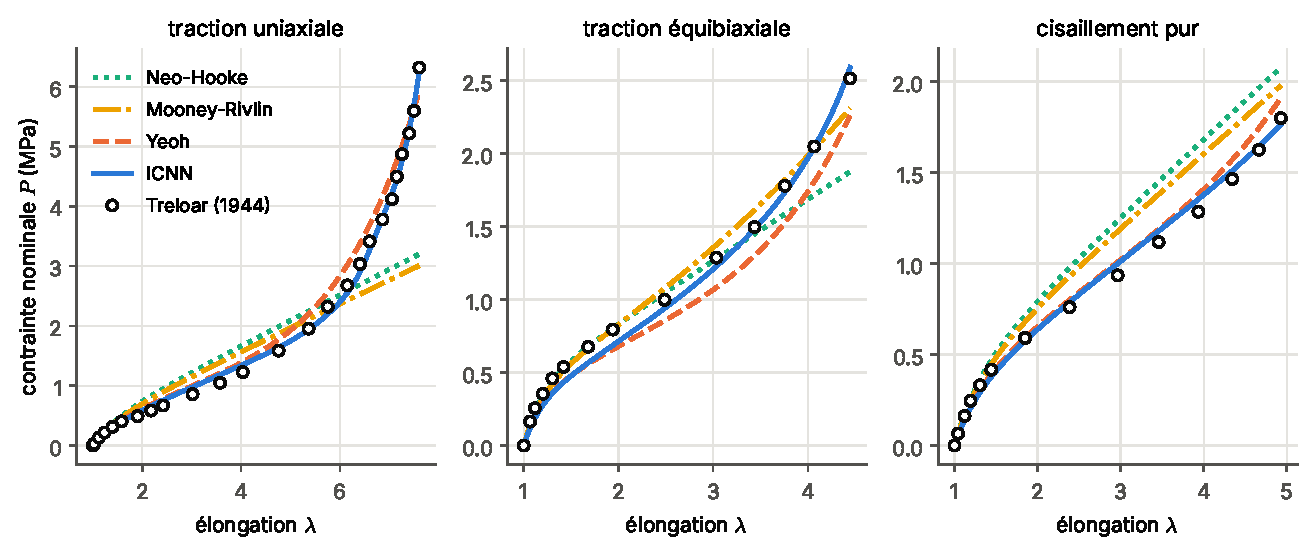
\includegraphics[width=\linewidth]{treloar_fit}
\caption{Identification sur les trois essais de Treloar.}\label{fig:treloar}
\end{figure}

\begin{figure}[h]
\centering
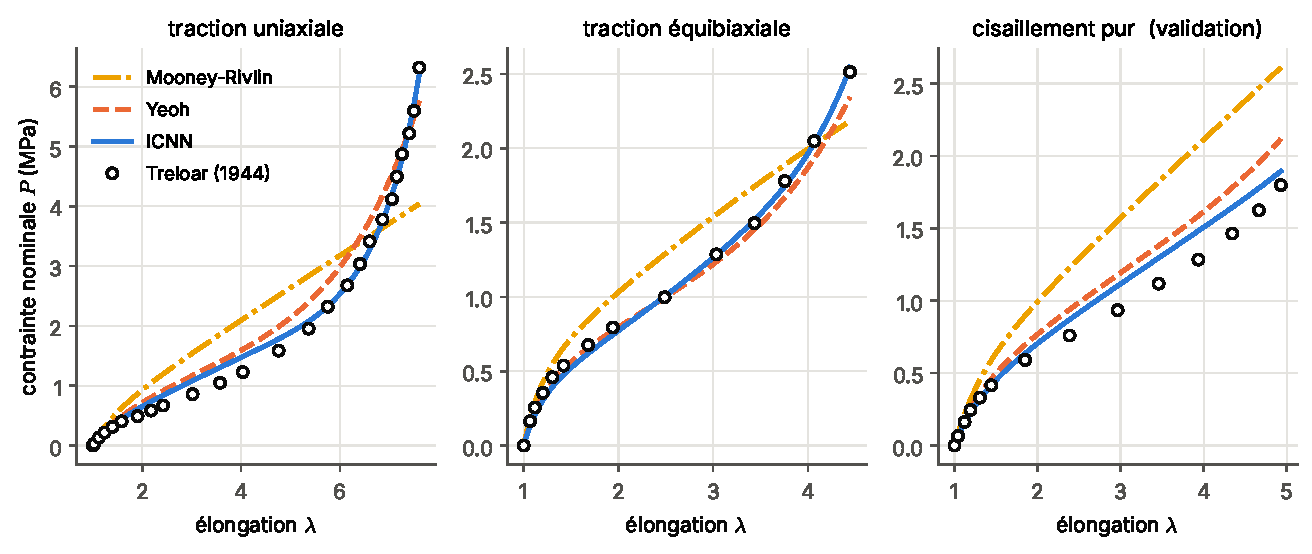
\includegraphics[width=\linewidth]{treloar_generalisation}
\caption{Identification sur UT et ET seulement. Le cisaillement pur (à droite) n'a pas servi à l'apprentissage.}\label{fig:treloar-gen}
\end{figure}

\begin{table}[h]
\centering
\begin{tabular}{l ccc ccc}
\toprule
 & \multicolumn{3}{c}{Apprentissage UT + ET + PS} & \multicolumn{3}{c}{Apprentissage UT + ET}\\
\cmidrule(lr){2-4}\cmidrule(lr){5-7}
Modèle & UT & ET & PS & UT & ET & PS (valid.)\\
\midrule
Neo-Hooke & $1{,}3\times10^{-1}$ & $2{,}8\times10^{-2}$ & $5{,}5\times10^{-2}$ & $8{,}0\times10^{-2}$ & $1{,}9\times10^{-2}$ & $2{,}6\times10^{-1}$\\
Mooney--Rivlin & $1{,}6\times10^{-1}$ & $3{,}7\times10^{-3}$ & $3{,}2\times10^{-2}$ & $7{,}5\times10^{-2}$ & $2{,}2\times10^{-2}$ & $3{,}0\times10^{-1}$\\
Yeoh & $5{,}3\times10^{-3}$ & $1{,}7\times10^{-2}$ & $4{,}7\times10^{-3}$ & $1{,}1\times10^{-2}$ & $3{,}1\times10^{-3}$ & $4{,}4\times10^{-2}$\\
ICNN & $\mathbf{8{,}4\times10^{-4}}$ & $\mathbf{3{,}6\times10^{-3}}$ & $\mathbf{1{,}7\times10^{-3}}$ & $\mathbf{1{,}7\times10^{-3}}$ & $\mathbf{1{,}1\times10^{-3}}$ & $\mathbf{1{,}4\times10^{-2}}$\\
\bottomrule
\end{tabular}
\caption{Erreur quadratique normalisée par essai (la racine donne l'ordre de l'erreur relative : $10^{-3}\leftrightarrow3\,\%$).}\label{tab:treloar}
\end{table}

\paragraph{Discussion.}
\begin{itemize}
  \item \textbf{Neo-Hooke et Mooney--Rivlin} ne reproduisent pas la remontée de la courbe uniaxiale au-delà de $\lambda\approx6$. Ce raidissement traduit l'extensibilité limitée des chaînes de polymère. Un potentiel linéaire en $I_1$ et $I_2$ ne peut pas le représenter : l'erreur relative en traction uniaxiale reste de 37 à 40\,\%.
  \item \textbf{Yeoh} capte la remontée grâce au terme cubique. Mais le coefficient identifié est $C_{20}<0$ : $\psi_1=C_{10}+2C_{20}x+3C_{30}x^2$ \emph{décroît} pour $x<7$, ce qui rend $\psi$ non convexe en $I_1$. La polyconvexité n'est plus garantie. C'est un défaut classique des polynômes identifiés sans contrainte.
  \item \textbf{L'ICNN} donne la meilleure précision sur les trois essais (erreur relative d'environ 3 à 6\,\%) \emph{et} garantit la polyconvexité. En validation sur le cisaillement pur, il prédit à environ 12\,\% près, contre 21\,\% pour Yeoh et 55\,\% pour Mooney--Rivlin. Les dérivées apprises sont physiquement lisibles : $\psi_1$ est presque constant jusqu'à $\lambda\approx5$ puis croît fortement (le raidissement), et $\psi_2$ est petit et positif (figure~\ref{fig:icnn-deriv}).
  \item \textbf{Limite.} La convexité interdit à $\psi_1$ de décroître. Or les données suggèrent une légère décroissance aux petites élongations, d'où la courbe légèrement au-dessus des points pour $2\le\lambda\le4$ en UT. Ce compromis est le prix de la garantie physique. Il peut être réduit avec $\psi_2$ et des invariants supplémentaires, comme dans les réseaux de type CANN~\cite{linka2021}.
\end{itemize}

\begin{figure}[h]
\centering
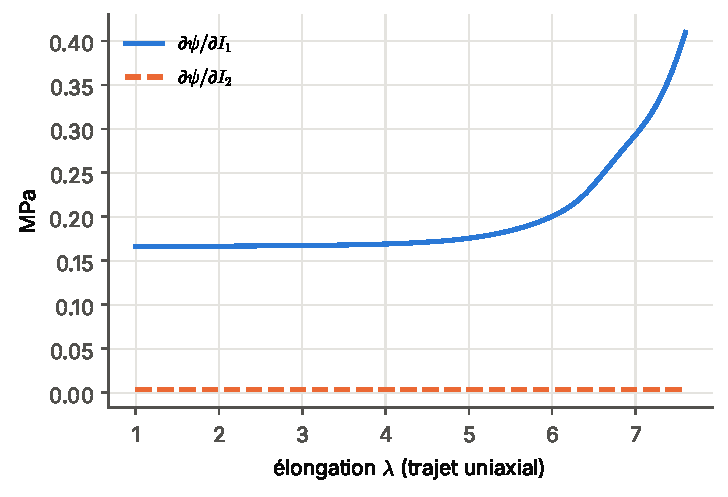
\includegraphics[width=0.55\linewidth]{treloar_icnn_derivatives}
\caption{Dérivées $\psi_1=\partial\psi/\partial I_1$ et $\psi_2=\partial\psi/\partial I_2$ de l'ICNN (scénario « tous ») le long du trajet uniaxial.}\label{fig:icnn-deriv}
\end{figure}
